\documentclass[a4paper,12pt]{article}
%%% Default imports
\usepackage{listings} % Code listings
\usepackage{graphicx} % Images
\usepackage{booktabs} % Better tables
\usepackage{makecell}
\usepackage{enumitem} % Lists
\usepackage{dsfont}
\usepackage{geometry} % Page geometry
\usepackage[utf8]{inputenc} % Encoding
\usepackage[T2A]{fontenc} % Font
\usepackage[english, russian]{babel} % Multi-language support
\usepackage{titling} % Better titles
\usepackage{textcomp} % Old-style numbers? Check difference
\usepackage{mathtext} % Russian text in math expressions? Check difference
\usepackage{amsmath, amsfonts, amssymb, amsthm, mathtools} % Mathematics
\usepackage{bm} % Bold math symbols
\usepackage{icomma} % Better comma in numbers within math mode
\usepackage{xifthen} % Better if-expressions
\usepackage{transparent} % Transparent colors
\usepackage{caption}    % }
\usepackage{subcaption} % } Captioning figures
\usepackage[table,xcdraw]{xcolor} % Colors
\usepackage{textpos} % Absolute positioning
\usepackage{upgreek} % Cool greek letters

\usepackage{fancyvrb}
\usepackage{fvextra}
\usepackage{chngcntr}

%%% Page geometry
\setlength\parindent{0pt} % No indentation between paragraphs
\setlist{noitemsep} % No spacing between list items

\usepackage{float}
\usepackage{multirow}

\geometry{
    paper=a4paper,
    top=2.5cm,
    bottom=3cm,
    left=2.5cm,
    right=2.5cm,
    headheight=0.75cm,
    footskip=1.5cm,
    headsep=0.75cm,
}

%%% Numeration
\newcommand{\RNumb}[1]{\uppercase\expandafter{\romannumeral #1\relax}}
\newcommand{\thesec}{\arabic{section}}
\renewcommand\thesection{\arabic{section}}
\renewcommand\thesubsection{\thesection.\arabic{subsection}}
\renewcommand\thesubsubsection{\RNumb{\arabic{subsubsection}}}
\renewcommand{\sectionmark}[1]{\markright{\thesection\ #1}}
\renewcommand{\bf}{\textbf}
\renewcommand{\it}{\textit}
\def\hash{\texttt{\#}}
\def\cpp{\C\texttt{++}}

\counterwithin{figure}{section}
\counterwithin{table}{section}
\renewenvironment{titlepage}{\thispagestyle{empty}} % Include titlepage into page numeration

%%% Headers and footers
\usepackage{setspace}
\usepackage{fancyhdr}
\usepackage{lastpage}


%%% Graphics
% Custom colors
\definecolor{myblue}{RGB}{72, 184, 178}
\definecolor{myblue1}{RGB}{0, 109, 167}
\definecolor{commentgreen}{RGB}{2,112,10}
\definecolor{mauve}{rgb}{0.58,0,0.82}
\definecolor{amethyst}{RGB}{153, 102, 203}

\usepackage{pgfplots} % Plots
\usepackage{tikz}
\usetikzlibrary{3d,perspective,decorations.text}
\usetikzlibrary{animations}
\usetikzlibrary{positioning}
\usetikzlibrary{matrix}
\usepackage{tikz-cd}
\usetikzlibrary{cd}
\usetikzlibrary{karnaugh}
\pgfplotsset{width=6cm,compat=newest}
\usepackage{color}

\usepackage[framemethod=TikZ]{mdframed}
\newcommand{\definebox}[2]{\newcounter{#1}\newenvironment{#1}[1][]{\stepcounter{#1}\mdfsetup{frametitle={\tikz[baseline=(current bounding box.east),outer sep=0pt]\node[anchor=east,rectangle,fill=white]{\strut \MakeUppercase#1~\csname the#1\endcsname\ifstrempty{##1}{}{:~##1}};}}\mdfsetup{innertopmargin=1pt,linecolor=#2,linewidth=3pt,topline=true,frametitleaboveskip=\dimexpr-\ht\strutbox\relax,}\begin{mdframed}[]\relax}{\end{mdframed}}}
\definebox{definition}{black!90}
\definebox{theorem}{myblue1!90}
\definebox{demonstration}{amethyst!90}

\newcounter{Theorem}
\def\themytheorem{\thesection.\arabic{Theorem}}
\usepackage[most]{tcolorbox}
\tcbuselibrary{theorems}
\newtcbtheorem{Theorem}{Theorem}
{colframe=myblue!90,coltitle=black,colback=white,fonttitle=\bfseries}{Th}

%%% Code listings
\usepackage{matlab-prettifier}

\lstdefinestyle{cpp} {
    language=C++,
    frame=tb,
    tabsize=4,
    showstringspaces=false,
    numbers=left,
    captionpos=b,
    columns=flexible,
    upquote=true,
    commentstyle=\color{commentgreen},
    keywordstyle=\color{blue},
    stringstyle=\color{commentgreen},
    basicstyle=\small\ttfamily,
    emph={int,char,double,float,unsigned,void,bool,size\_t},
    emphstyle={\color{blue}},
    escapechar=\&,
    classoffset=1,
    otherkeywords={>,<,.,;,-,!,=,~},
    morekeywords={>,<,.,;,-,!,=,~},
    keywordstyle=\color{black},
    classoffset=0,
}
\lstdefinestyle{def} {
    frame=tb,
    tabsize=4,
    showstringspaces=false,
    numbers=left,
    captionpos=b,
    columns=flexible,
    upquote=true,
    commentstyle=\color{black},
    keywordstyle=\color{black},
    stringstyle=\color{black},
    basicstyle=\small\ttfamily,
    emph={int,char,double,float,unsigned,void,bool,size\_t},
    emphstyle={\color{black}},
    escapechar=\&,
    classoffset=1,
    otherkeywords={>,<,.,;,-,!,=,~},
    morekeywords={>,<,.,;,-,!,=,~},
    keywordstyle=\color{black},
    classoffset=0,
}
\lstdefinelanguage[RISC-V]{Assembler}
{
    alsoletter={.}, % allow dots in keywords
    alsodigit={0x}, % hex numbers are numbers too!
    morekeywords=[1]{ % instructions
    lb, lh, lw, lbu, lhu,
    sb, sh, sw,
    sll, slli, srl, srli, sra, srai,
    add, addi, sub, lui, auipc,
    xor, xori, or, ori, and, andi,
    slt, slti, sltu, sltiu,
    beq, bne, blt, bge, bltu, bgeu,
    j, jr, jal, jalr, ret,
    scall, break, nop
},
    morekeywords=[2]{ % sections of our code and other directives
    .align, .ascii, .asciiz, .byte, .data, .double, .extern,
    .float, .globl, .half, .kdata, .ktext, .set, .space, .text, .word
},
    morekeywords=[3]{ % registers
    zero, ra, sp, gp, tp, s0, fp,
    t0, t1, t2, t3, t4, t5, t6,
    s1, s2, s3, s4, s5, s6, s7, s8, s9, s10, s11,
    a0, a1, a2, a3, a4, a5, a6, a7,
    ft0, ft1, ft2, ft3, ft4, ft5, ft6, ft7,
    fs0, fs1, fs2, fs3, fs4, fs5, fs6, fs7, fs8, fs9, fs10, fs11,
    fa0, fa1, fa2, fa3, fa4, fa5, fa6, fa7
},
    morecomment=[l]{;},   % mark ; as line comment start
    morecomment=[l]{\#},  % as well as # (even though it is unconventional)
    morestring=[b]",      % mark " as string start/end
    morestring=[b]'       % also mark ' as string start/end
}
\lstdefinestyle{riscv} {
    basicstyle=\small\ttfamily,                    % very small code
    breaklines=true,                              % break long lines
    commentstyle=\itshape\color{green!50!black},  % comments are green
    keywordstyle=[1]\color{blue!80!black},        % instructions are blue
    keywordstyle=[2]\color{orange!80!black},      % sections/other directives are orange
    keywordstyle=[3]\color{red!50!black},         % registers are red
    stringstyle=\color{mauve},                    % strings are from the telekom
    identifierstyle=\color{teal},                 % user declared addresses are teal
    frame=l,                                      % black line on the left side of code
    captionpos=b,
    language=[RISC-V]Assembler,                   % all code is RISC-V
    tabsize=4,                                    % indent tabs with 4 spaces
    showstringspaces=false                        % do not replace spaces with weird underlines
}

%%% Other
\usepackage[normalem]{ulem} % }
\useunder{\uline}{\ul}{}    % } Underline text
\usepackage[colorlinks,urlcolor=blue,filecolor=blue,citecolor=blue,linkcolor = blue,unicode=true]{hyperref}
\usepackage{titlesec}
\titlelabel{\thetitle.\quad}
\usepackage{secdot}
\sectiondot{subsection}
\usepackage{kvmap} % Karnaugh-maps for logic functions
\usepackage{}
\newcommand{\projectname}[3]{
    \begin{center}
        \Large
        \textbf{#1}\\[10pt]
        \textbf{#2}\\[10pt]
        \normalsize
        #3
        \rule{\linewidth}{0.4pt}
    \end{center}
}

\newcommand{\hfconfiguration}[3]{
    \pagestyle{fancy}
    \fancyhead[LE,RO]{}
    \fancyhead[LO,RE]{#1}
    \renewcommand{\footrulewidth}{0.4pt}
    \fancyfoot[C]{\thepage/\pageref*{LastPage}}
    \fancyfoot[LO,RE]{#2}
    \fancyfoot[LE,RO]{#3}
}

\newcommand{\filename}[2]{
    \pagebreak
    \titleformat{\section}
    [display]
    {\bfseries\Large}
    {}
    {0ex}
    {
        \vspace{-4.5ex}
        % \rule{\textwidth}{1pt}
        #1 \centering
    % \vspace{1ex}
    }
    [
        \normalfont\large
        #2
        \rule{\textwidth}{0.4pt}
        \normalsize
    ]
}

\newcommand{\project}[6]{
    \projectname{#1}{#2}{#3}
    \pagestyle{empty}
    \tableofcontents
    \newpage
    \hfconfiguration{#4}{#5}{#6}
}
%%% Final touch
\usepackage{subfiles}


\begin{document}
    \begin{titlepage}
    \begin{center}
        \large Санкт-Петербургский политехнический университет Петра Великого\\
        \large Институт компьютерных наук и технологий \\
        \large Кафедра компьютерных систем и программных технологий\\[6cm]


        \huge Отчет по лабораторной работе №4\\[0.5cm]
        \large по дисциплине <<Схемотехника операционных устройств>>\\[0.1cm]
        \large\textbf{Синтез конечных автоматов}\\[5cm]
    \end{center}


    \begin{flushright}
        \begin{minipage}{0.25\textwidth}
            \begin{flushleft}

                \large\textbf{Работу выполнил:}\\
                \large Ильин В.П.\\
                \large {Группа:} 35300901/10005\\

                \large \textbf{Преподаватель:}\\
                \large Киселев И.О.

            \end{flushleft}
        \end{minipage}
    \end{flushright}

    \vfill

    \begin{center}
        \large Санкт-Петербург\\
        \large \the\year
    \end{center}
\end{titlepage}

\vfill
\newpage

    \tableofcontents
    \hfconfiguration{Лабораторная работа №4}{}{}

    \section{Цели работы}
    \begin{itemize}
        \item Закрепление навыков структурного синтеза конечных автоматов;
        \item Закрепление знаний о характеристиках и режимах работы триггеров основных типов;
        \item Получение практических навыков тестирования и управления КА;
        \item Получение навыков ввода прокта в графическом редакторе пакета QP,
        тестирования и отладки проекта и анализа временных характеристик КА;
        \item Знакомство с редактором КА пакета QP  и анализ результатов синтеза;
        \item Получение навыков отладки цифровых устройств класса КА на физической модели:
        конфигурирование ПЛИС и экспериментальная проверка работы КА при использовании
        лабораторного стенда.
    \end{itemize}
    \section{Исходные данные}
    Вариант исходного задания -- 8. Тип триггера -- JK.

    \begin{minipage}{0.5\linewidth}
        \begin{table}[H]
            \centering
            \begin{tabular}{|cl|cccc|}
            \hline
            \multicolumn{2}{|c|}{\multirow{2}{*}{$(x_2, x_1)^t$}} & \multicolumn{4}{c|}{$r^t$}                                                   \\ \cline{3-6} 
            \multicolumn{2}{|c|}{}                                & \multicolumn{1}{c|}{0} & \multicolumn{1}{c|}{1} & \multicolumn{1}{c|}{2} & 3 \\ \hline
            \multicolumn{2}{|c|}{0 0}                             & \multicolumn{1}{c|}{2} & \multicolumn{1}{c|}{H} & \multicolumn{1}{c|}{0} & 1 \\ \hline
            \multicolumn{2}{|c|}{0 1}                             & \multicolumn{1}{c|}{H} & \multicolumn{1}{c|}{H} & \multicolumn{1}{c|}{H} & H \\ \hline
            \multicolumn{2}{|c|}{1 0}                             & \multicolumn{1}{c|}{3} & \multicolumn{1}{c|}{0} & \multicolumn{1}{c|}{H} & 2 \\ \hline
            \multicolumn{2}{|c|}{1 1}                             & \multicolumn{1}{c|}{H} & \multicolumn{1}{c|}{2} & \multicolumn{1}{c|}{3} & 1 \\ \hline
            \end{tabular}
            \caption{Таблица переходов}
            \label{tab:transtab}
        \end{table}
    \end{minipage}
    \begin{minipage}[b]{0.5\linewidth}
        \begin{table}[H]
            \centering
            \begin{tabular}{|c|c|c|c|c|}
            \hline
            $r^t$          & 0  & 1  & 2  & 3  \\ \hline
            $(y_2, y_1)^t$ & 01 & 10 & 10 & 01 \\ \hline
            \end{tabular}
            \caption{Таблица выходов}
        \end{table}
    \end{minipage}

    \newpage
    \section{Ход работы}
    \subsection{Структурный синтез КА}
    При помощи таблицы~\ref{tab:transtab} составим граф переходов.

    \begin{figure}[H]
    \begin{center}
        \begin{tikzpicture}[
            nodecirc/.style={circle, draw=black, fill=gray!30, thick},
            nofill/.style={circle, draw=cyan},
            filled/.style={circle, draw=cyan, fill=cyan}
        ]
        \matrix (m) [ matrix of nodes, row sep=2cm, column sep=4cm,
                    nodes = {anchor=center}] {
                    |[nodecirc]{$r_0$};| & |[nodecirc]{$r_1$};| \\
                    |[nodecirc]{$r_3$};| & |[nodecirc]{$r_2$};| \\
        };
        \draw[->, thick] (m-1-1) to node[left] {10} (m-2-1);
        \draw[->, thick] (m-1-2) to node[above] {10} (m-1-1);
        \draw[->, thick] (m-1-2) to node[right] {11} (m-2-2);
        \draw[->, thick] (m-2-2) to node[above] {11} (m-2-1);
        \def\myshift#1{\raisebox{-2.5ex}}
        \draw [->,thick,postaction={decorate,decoration={text along path,text align=center,text={|\myshift|10}}}] (m-2-1) to [bend right=15]  (m-2-2);
        \draw [->,thick,postaction={decorate,decoration={text along path,text align=center,text={|\myshift|00}}}] (m-2-1) to [bend right=5]  (m-1-2);
        \def\myshift#1{\raisebox{1ex}}
        \draw [->,thick,postaction={decorate,decoration={text along path,text align=center,text={|\myshift|11}}}] (m-2-1) to [bend right=-5]  (m-1-2);
        \draw[<->, thick, red] (m-2-2) to node[right] {00} (m-1-1);
        \end{tikzpicture}
        \caption{Граф переходов синтезируемого автомата}
    \end{center}
\end{figure}
    Всего автомат имеет 4 различных состояния, значит, минимальное необходиоме число триггеров $m = \log_2 4 = 2$.
    Воспользовавшись экономичным кодированием внутренних состояний, получим необходимые коды:
    \begin{table}[H]
        \centering
        \begin{tabular}{|c|c|c|c|c|}
        \hline
        $r^t$          & 0  & 1  & 2  & 3  \\ \hline
        $(Q_2, Q_1)^t$ & 00 & 01 & 11 & 10 \\ \hline
        \end{tabular}
        \caption{Коды состояний автомата}
        \label{tab:statecodes}
    \end{table}
    Воспользовавшись таблицами~\ref{tab:transtab} и~\ref{tab:statecodes} получим закодированную таблицу
    переходов синтезируемого КА:
    \begin{table}[H]
        \centering
        \begin{tabular}{|cl|cccc|}
        \hline
        \multicolumn{2}{|c|}{\multirow{2}{*}{$(x_2, x_1)^t$}} & \multicolumn{4}{c|}{$(Q_2, Q_1)^t$}                                                   \\ \cline{3-6} 
        \multicolumn{2}{|c|}{}                                & \multicolumn{1}{c|}{00} & \multicolumn{1}{c|}{01} & \multicolumn{1}{c|}{11} & 10 \\ \hline
        \multicolumn{2}{|c|}{0 0}                             & \multicolumn{1}{c|}{11} & \multicolumn{1}{c|}{H} & \multicolumn{1}{c|}{00} & 01 \\ \hline
        \multicolumn{2}{|c|}{0 1}                             & \multicolumn{1}{c|}{H} & \multicolumn{1}{c|}{H} & \multicolumn{1}{c|}{H} & H \\ \hline
        \multicolumn{2}{|c|}{1 0}                             & \multicolumn{1}{c|}{10} & \multicolumn{1}{c|}{00} & \multicolumn{1}{c|}{H} & 11 \\ \hline
        \multicolumn{2}{|c|}{1 1}                             & \multicolumn{1}{c|}{H} & \multicolumn{1}{c|}{11} & \multicolumn{1}{c|}{10} & 01 \\ \hline
        \end{tabular}
        \caption{Таблица переходов}
        \label{tab:transtab_coded}
    \end{table}    
    Используя таблицу истинности для JK-триггера, построим таблицу управления триггером:
    \begin{table}[H]
        \centering
        \begin{tabular}{|c|c|c|c|c|c|c|}
        \hline
        $(x_2, x_1)^t$ & $(Q_2, Q_1)^t$ & $(Q_2, Q_1)^{t+1}$ & $J_2$ & $K_2$ & $J_1$ & $K_1$ \\ \hline
        00             & 00             & 11                 & 1     & H     & 1     & H     \\ \hline
        00             & 01             & H                  & H     & H     & H     & H     \\ \hline
        00             & 11             & 00                 & H     & 1     & H     & 1     \\ \hline
        00             & 10             & 01                 & H     & 1     & 1     & H     \\ \Xhline{4\arrayrulewidth}
        01             & 00             & H                  & H     & H     & H     & H     \\ \hline
        01             & 01             & H                  & H     & H     & H     & H     \\ \hline
        01             & 11             & H                  & H     & H     & H     & H     \\ \hline
        01             & 10             & H                  & H     & H     & H     & H     \\ \Xhline{4\arrayrulewidth}
        10             & 00             & 10                 & 1     & H     & 0     & H     \\ \hline
        10             & 01             & 00                 & 0     & H     & H     & 1     \\ \hline
        10             & 11             & H                  & H     & H     & H     & H     \\ \hline
        10             & 10             & 11                 & H     & 0     & 1     & H     \\ \Xhline{4\arrayrulewidth}
        11             & 00             & H                  & H     & H     & H     & H     \\ \hline
        11             & 01             & 11                 & 1     & H     & H     & 0     \\ \hline
        11             & 11             & 10                 & H     & 0     & H     & 1     \\ \hline
        11             & 10             & 01                 & H     & 1     & 1     & H     \\ \hline
        \end{tabular}
        \caption{Таблица функций возбуждения триггеров}
        \label{tab:erection}
    \end{table}
    Произведем минимизацию полученных функций при помощи карт Карно:

    \begin{minipage}{0.5\linewidth}
        \begin{center}
            \begin{tikzpicture}[karnaugh,
                thick,
                grp/.style n args={3}{#1,fill=#1!30,
                    minimum width=#2\kmunitlength,
                    minimum height=#3\kmunitlength,
                    rounded corners=0.2\kmunitlength,
                    fill opacity=0.6,
                    rectangle,draw}]]
                \karnaughmaptab{4}{$J_2$}{{$x_2$}{$x_1$}{$Q_2$}{$Q_1$}}%
                {1HHH HHHH H1HH 10HH}%
                {
                    \node[grp={blue}{0.9}{3.9}](n000) at (0.5, 2.0) {};
                    \node[grp={red}{3.9}{1.9}](n001) at (2.0, 2.0) {};
                }
            \end{tikzpicture}
        
            $J_2 = \color{blue}\overline{Q}_1 \overline{Q_2} \color{black} + \color{red} x_1 \color{black} = \overline{\overline{x}_1 \overline{\overline{Q}_1 \overline{Q}_2}}$
        \end{center}
    \end{minipage}
    \begin{minipage}{0.5\linewidth}
        \begin{center}
            \begin{tikzpicture}[karnaugh,
                thick,
                grp/.style n args={3}{#1,fill=#1!30,
                    minimum width=#2\kmunitlength,
                    minimum height=#3\kmunitlength,
                    rounded corners=0.2\kmunitlength,
                    fill opacity=0.6,
                    rectangle,draw}]]
                \karnaughmaptab{4}{$K_2$}{{$x_2$}{$x_1$}{$Q_2$}{$Q_1$}}%
                {HH11 HHHH HH01 HHH0}%
                {
                    \node[grp={blue}{3.9}{1.9}](n001) at (2.0, 3.0) {};
                    \node[grp={red}{0.9}{1.9}](n000) at (3.5, 2.0) {};
                    \node[grp={red}{0.9}{1.9}](n002) at (0.5, 2.0) {};
                }
            \end{tikzpicture}
        
            $K_2 = \color{blue}\overline{x}_2 \color{black} + \color{red} x_1\overline{Q}_1 \color{black} = \overline{x_2 \overline{x_1 \overline{Q}_1}}$
        \end{center}
    \end{minipage}

    \begin{minipage}{0.5\linewidth}
        \begin{center}
            \begin{tikzpicture}[karnaugh,
                thick,
                grp/.style n args={3}{#1,fill=#1!30,
                    minimum width=#2\kmunitlength,
                    minimum height=#3\kmunitlength,
                    rounded corners=0.2\kmunitlength,
                    fill opacity=0.6,
                    rectangle,draw}]]
                \karnaughmaptab{4}{$J_1$}{{$x_2$}{$x_1$}{$Q_2$}{$Q_1$}}%
                {1HH1 HHHH HHH1 0HH1}%
                {
                    \node {};
                    \node[grp={blue}{3.9}{1.9}](n001) at (2.0, 3.0) {};
                    \node[grp={red}{1.9}{3.9}](n000) at (3.0, 2.0) {};
                }
            \end{tikzpicture}
        
            $J_1 = \color{blue}\overline{x}_2 \color{black} + \color{red} Q_2 \color{black} = \overline{x_2 \overline{Q}_2}$
        \end{center}
    \end{minipage}
    \begin{minipage}{0.5\linewidth}
        \begin{center}
            \begin{tikzpicture}[karnaugh,
                thick,
                grp/.style n args={3}{#1,fill=#1!30,
                    minimum width=#2\kmunitlength,
                    minimum height=#3\kmunitlength,
                    rounded corners=0.2\kmunitlength,
                    fill opacity=0.6,
                    rectangle,draw}]]
                \karnaughmaptab{4}{$K_1$}{{$x_2$}{$x_1$}{$Q_2$}{$Q_1$}}%
                {HH1H HHHH H01H H1HH}%
                {
                    \node {};
                    \node[grp={blue}{3.9}{0.9}](n001) at (2.0, 3.5) {};
                    \node[grp={blue}{3.9}{0.9}](n002) at (2.0, 0.5) {};
                    \node[grp={red}{1.9}{3.9}](n000) at (3.0, 2.0) {};
                }
            \end{tikzpicture}
        
            $K_1 = \color{blue}\overline{x}_1 \color{black} + \color{red} Q_2 \color{black} = \overline{x_1 \overline{Q}_2}$
        \end{center}
    \end{minipage}

    Также составим таблицу для выходных сигналов, как функций состояния автоматов, и проведем минимизацию.
    \begin{table}[H]
        \centering
        \begin{tabular}{|c|c|}
        \hline
        $(Q_2, Q_1)$ & $(y_2, y_1)$ \\ \hline
        0 0          & 0 1          \\ \hline
        0 1          & 1 0          \\ \hline
        1 1          & 1 0          \\ \hline
        1 0          & 0 1          \\ \hline
        \end{tabular}
    \end{table}
    \[y_1 = \overline{Q}_1, \, y_2 = Q_2 \overline{Q}_1 + \overline{Q}_2 Q_1 = \overline{\overline{Q_2 \overline{Q}_1} \cdot \overline{\overline{Q}_2 Q_1}}\]

    \subsection{Исследование синтезированного автомата}
    Введем схему синтезированного автомата в Quartus Prime.
    \begin{figure}[H]
        \centering
        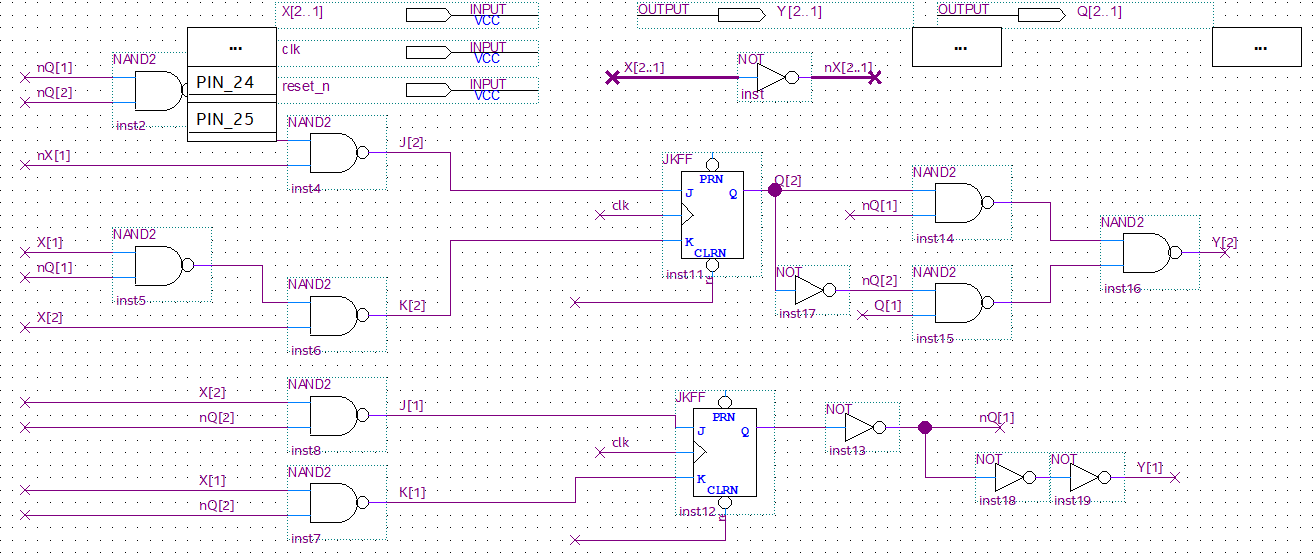
\includegraphics[width=\linewidth]{polytech/scheme/report-lab4/subfiles/images/scheme}
        \caption{Синтезированная схема}
        \label{fig:scheme}
    \end{figure}
    \begin{figure}[H]
        \centering
        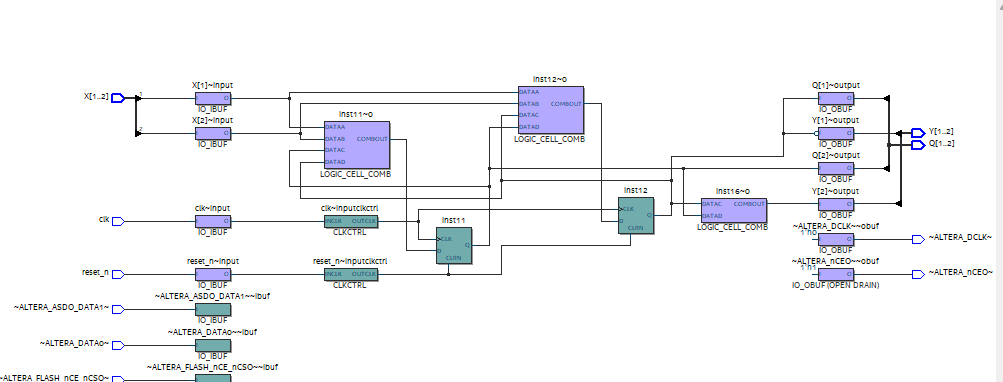
\includegraphics[width=\linewidth]{polytech/scheme/report-lab4/subfiles/images/tmv1}
        \caption{Technology Map Viewer}
        \label{fig:tmv1}
    \end{figure}
    \begin{figure}[H]
        \centering
        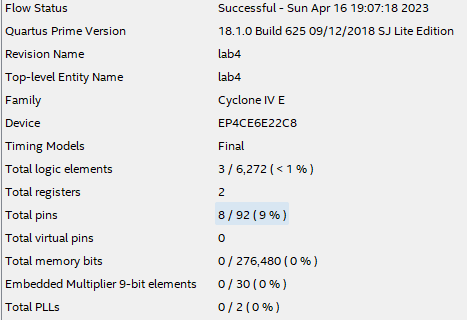
\includegraphics[width=.7\linewidth]{polytech/scheme/report-lab4/subfiles/images/app}
        \caption{Аппаратные затраты}
        \label{fig:app}
    \end{figure}
    \begin{figure}[H]
        \centering
        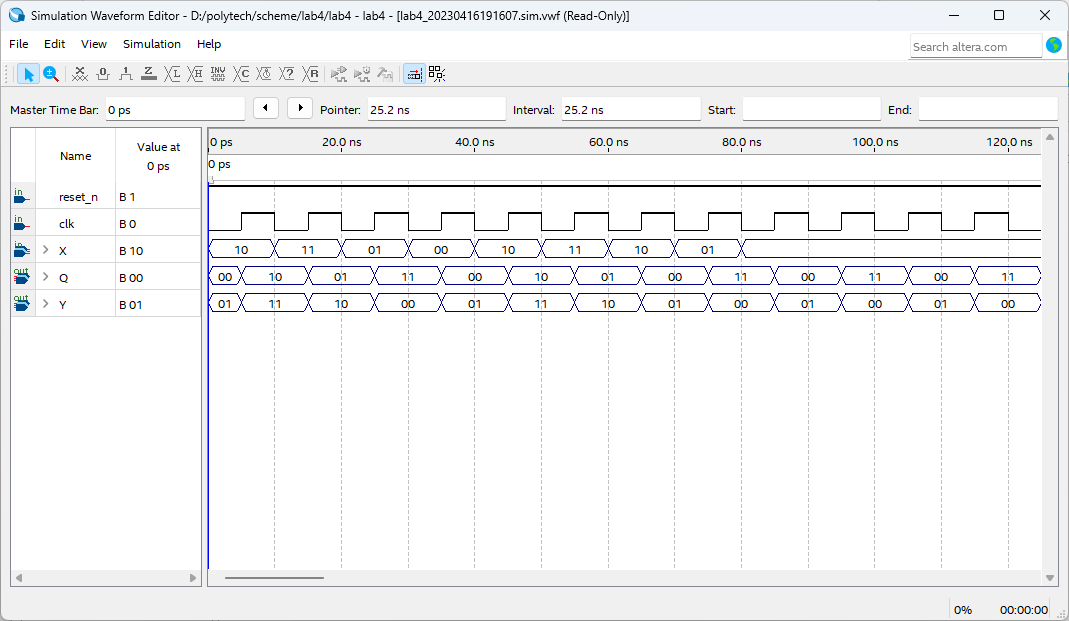
\includegraphics[width=\linewidth]{polytech/scheme/report-lab4/subfiles/images/wave}
        \caption{Моделирование работы}
        \label{fig:wave}
    \end{figure}

    Сравнение выходных результатов для Q и Y подтверждает правильность работы устройства.

    \subsection{Синтез конечного автомата средствами Quartus Prime}

    Теперь создадим автомат при помощи встроенных средств среды Quartus.

    \begin{figure}[H]
        \centering
        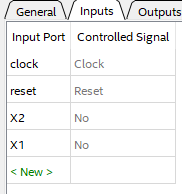
\includegraphics[width=0.25\linewidth]{polytech/scheme/report-lab4/subfiles/images/smw1}
        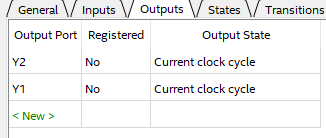
\includegraphics[width=0.4\linewidth]{polytech/scheme/report-lab4/subfiles/images/smw2}
        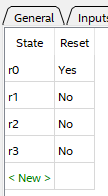
\includegraphics[width=0.15\linewidth]{polytech/scheme/report-lab4/subfiles/images/smw3}

        \begin{minipage}{0.45\linewidth}
            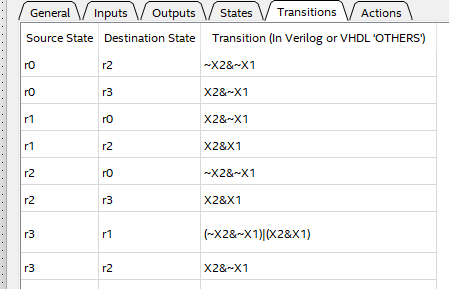
\includegraphics[width=\linewidth]{polytech/scheme/report-lab4/subfiles/images/smw4}
        \end{minipage}
        \begin{minipage}{0.45\linewidth}
            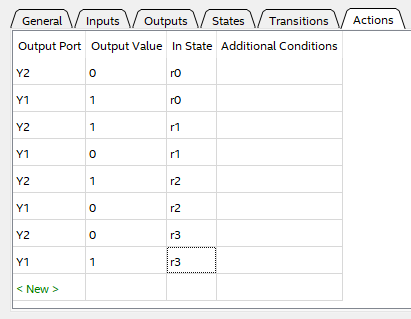
\includegraphics[width=\linewidth]{polytech/scheme/report-lab4/subfiles/images/smw5}
        \end{minipage}
        \caption{Настройки создания автомата}
    \end{figure}

    \begin{figure}[H]
        \centering
        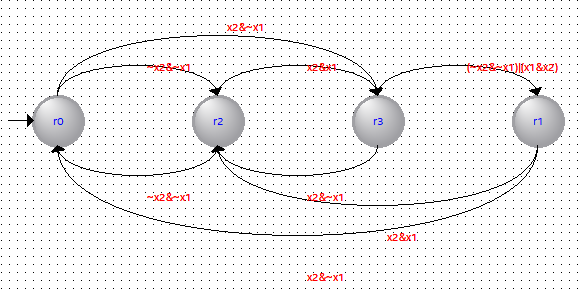
\includegraphics[width=\linewidth]{polytech/scheme/report-lab4/subfiles/images/scheme_machine}
        \caption{Синтезированная схема}
    \end{figure}
    \begin{figure}[H]
        \centering
        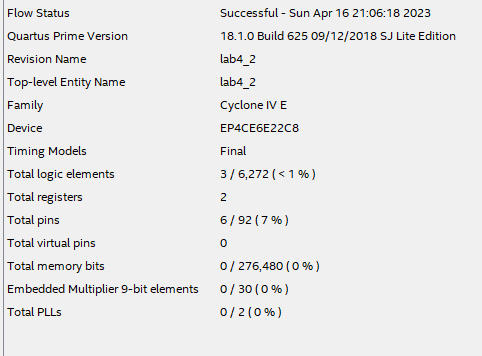
\includegraphics[width=0.7\linewidth]{polytech/scheme/report-lab4/subfiles/images/compile_machine}
        \caption{Отчет о компиляции}
    \end{figure}
    \begin{figure}[H]
        \centering
        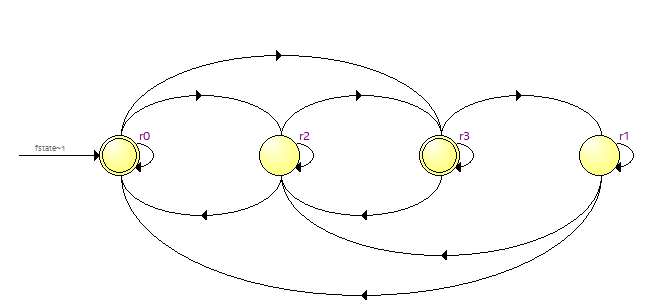
\includegraphics[width=\linewidth]{polytech/scheme/report-lab4/subfiles/images/smv}
        \caption{State Machine Viewer}
    \end{figure}
    \section{Вывод}
    В ходе работы были закреплены знания характеристик и режимов работы триггеров. Были получены навыки
    структурного синтеза, тестирования и управления конечными автоматами. Конечный автомат на основе заданных
    данных был синтезирован вручную, а также при помощи встроенных средств Quartus Prime. Автомат, полученный
    вручную работает медленее и содержит большее число элементов, чем созданный автоматически. Помимо оптимизаций,
    производимых Quartus это также связано с тем, что для тестирования <<ручной>> автомат выводил промежуточные значения.
\end{document}
